\documentclass[12pt,a4paper]{report}
\usepackage{vntex} % Tiếng Việt
\usepackage{graphicx} % Chèn hình ảnh
\usepackage{fancyhdr} % Gói hỗ trợ tạo header và footer fancy
\usepackage{changepage} % Thay đổi lề
\usepackage{pdfpages} % Chèn pdf
% Chèn code
\usepackage{listings} % Thêm gói listings để chèn code
\usepackage{xcolor} % Màu cho code
\lstset{
    language=R,
    basicstyle=\footnotesize\ttfamily,
    numbers=none,
    numberstyle=\tiny\color{gray},
    stepnumber=1,
    numbersep=0.01pt,
    tabsize=2,
    breaklines=true,
    breakatwhitespace=false,
    xleftmargin=0cm, % for line numbers
    framexleftmargin=0cm, % for code frame
    keywordstyle=\color{blue},
    commentstyle=\color{green},
    stringstyle=\color{orange},
    frame=single,
    rulecolor=\color{black},
    basicstyle=\ttfamily,
}
% Thiết lập bảng
\usepackage{array} % Gói hỗ trợ các bảng phức tạp
\usepackage{tabularx}
\usepackage{longtable} % Tạo bảng qua nhiều trang
\usepackage{cellspace}
\usepackage{diagbox} % Gói hỗ trợ tạo các ô chéo trong bảng

% Thiết lập công thức toán học
\usepackage{amsmath} % Gói hỗ trợ các công thức toán học
\usepackage{amsfonts} % Gói hỗ trợ các ký hiệu toán học
\usepackage{amssymb} % Gói hỗ trợ các ký hiệu toán học
\usepackage{graphicx} % Gói hỗ trợ chèn hình ảnh
\usepackage{bm} % Chữ in đậm trong công thức toán 

% Thiết lập khác
\usepackage{tikz}
\usepackage{color}
\usepackage{subcaption}
\usepackage{framed}
\usepackage{float} % Để chèn hình ảnh vào đúng vị trí
\usepackage{fancyvrb} % Đưa dữ liệu dạng nguyên thủy vào


% Thiết lập kích thước
\usepackage{geometry}
\geometry{
    left=3cm,
    right=2cm,
    top=2.5cm,
    bottom=2.5cm,
}
\usepackage{hyperref} %Chèn link
\hypersetup{urlcolor=black,linkcolor=black,citecolor=black,colorlinks=true} % Màu cho các đường nét
\everymath{\color{black}}
\setlength{\headheight}{40pt}
\pagestyle{fancy}

\renewcommand{\thesection}{\arabic{section}} %Định dạng cho số của section
\renewcommand{\thesubsection}{\thesection.\arabic{subsection}}
%Header
\fancyhead{} % clear all header fields
\fancyhead[L]{
 \begin{tabular}{rl}
    \begin{picture}(25,15)(0,0)
    \put(0,-8){
\includegraphics[width=12mm, height=12mm]{pictures/hcmut.png}}
    %\put(0,-8){\epsfig{width=10mm,figure=hcmut.eps}}
   \end{picture}&
	%
\includegraphics[width=8mm, height=8mm]{hcmut.png} & %
	\begin{tabular}{l}
		\textbf{\bf \ttfamily Trường Đại Học Bách Khoa - ĐHQG TP.Hồ Chí Minh}\\
		\textbf{\bf \ttfamily Khoa Cơ Khí - Bộ môn Thiết kế máy}
	\end{tabular} 	
 \end{tabular}
}
\fancyhead[R]{
	{\tiny \bf \quad} % Khoảng trắng nhỏ trong header bên phải
}

%Footer
\fancyfoot{} % clear all footer fields
\fancyfoot[L]{\scriptsize \ttfamily Đồ án hệ thống truyền động}
\fancyfoot[R]{\scriptsize \ttfamily Trang {\thepage}/4}
\renewcommand{\headrulewidth}{0.3pt}
\renewcommand{\footrulewidth}{0.3pt}
\begin{document}
    \begin{titlepage}   
    \begin{center}
        \vspace*{-2cm} 
        \large
        \textbf{ĐẠI HỌC QUỐC GIA THÀNH PHỐ HỒ CHÍ MINH \\
        TRƯỜNG ĐẠI HỌC BÁCH KHOA\\
        KHOA CƠ KHÍ\\
        BỘ MÔN THIẾT KẾ MÁY}\\
        
\includegraphics[width=70mm, height=70mm]{pictures/hcmut.png} \\
        \rule{\linewidth}{0.5mm}\\
        \vspace{0.8cm}
        \Large
        \textbf{BÁO CÁO ĐỒ ÁN}\\
        \vspace*{0.5cm}
        \Huge
        \textbf{HỆ THỐNG TRUYỀN ĐỘNG}\\
        \vspace{0.5cm}
        \rule{\linewidth}{0.5mm}\\
        \vspace{0.8cm}
        \vspace{1cm}
        \large
        \textbf{GVHD: THẦY PHẠM MINH TUẤN}\\
        \vspace{0.5cm}
        LỚP: TN01 \\
        \vspace{0.5cm}
        SINH VIÊN THỰC HIỆN:\\[0.3cm]
        \begin{tabular}{|>{\centering\arraybackslash}m{7cm}|>{\centering\arraybackslash}m{5cm}|>{\centering\arraybackslash}m{5cm}|}
            \hline
             \textbf{Họ và tên} & \textbf{MSSV} \\
            \hline
             Dương Quang Duy & 2210497 \\
            \hline
            Đoàn Nguyễn Minh Khoa & 2211586 \\
            \hline
        \end{tabular}
    \end{center}
        
    \vfill
    \large
    \begin{center}
        TP.HCM, \today
    \end{center}
\end{titlepage}

    \tableofcontents
    \cleardoublepage
    \thispagestyle{empty}
\begin{center}
    \textbf{\Large{ĐỀ SỐ 4: THIẾT KẾ HỆ THỐNG TRUYỀN ĐỘNG MÁY ÉP BÙN}}\\
    \textbf{\Large{PHƯƠNG ÁN 6}}\\

\end{center}
\begin{figure}[H]
    \centering
    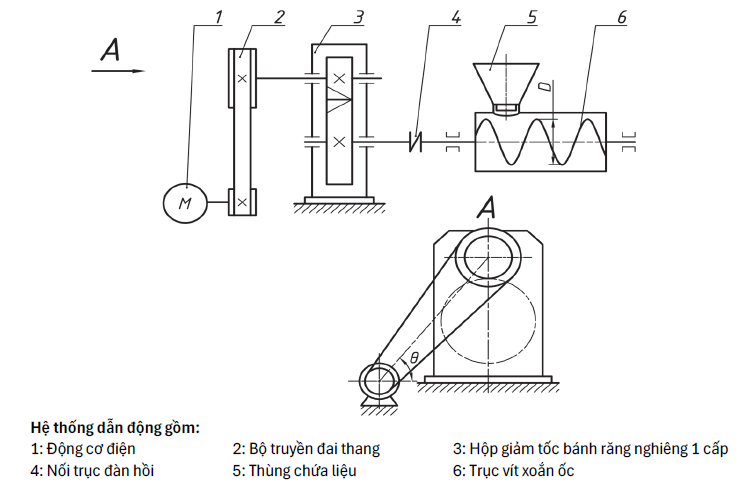
\includegraphics[width=1\textwidth]{pictures/debai.png}
\end{figure}
\begin{center}
\begin{tabular}{|c|c|}
    \hline
    \textbf{Phương án} & \textbf{6} \\
    \hline
    Lực vòng trên cánh vít F, (N) & 2800  \\
    \hline     
    Vận tốc vòng cánh vít v, (m/s) & 1,3  \\
    \hline
    Đường kính cánh vít, D (mm) & 225  \\
    \hline
    Thời gian phục vụ L, (năm) & 7  \\
    \hline
    Số ca làm việc, (ca) & 2  \\
    \hline
    Thời gian làm việc mỗi ca, (giờ) & 8  \\
    \hline
    Số giờ làm việc mỗi năm, (giờ) & 300  \\
    \hline
\end{tabular}
\end{center}
\cleardoublepage
    \chapter{Chọn động cơ điện}
\section{Xác định công suất bộ phận công tác}
\begin{equation}
    P_{ct} = \frac{F.v}{1000} = \frac{2800 \cdot 1.4}{1000} = 3.92 \, \text{kW}
\end{equation}

\section{Số vòng quay của bộ phận công tác}
\begin{equation}
    n_{ct} = \frac{60000.v}{\pi.D} = \frac{60000 \cdot 1.4}{\pi \cdot 225} = 118.84 \, \text{(v/ph)}
\end{equation}

\section{Hiệu suất của các bộ truyền và các cặp ổ trong hệ thống dẫn động}
\begin{itemize}
    \item Bộ truyền đai: $\eta_{d} = 0.96$ 
    \item Bộ truyền bánh răng: $\eta_{br} = 0.98$
    \item Nối trục: $\eta_{nt} = 0.99$
    \item Ổ lăn: $\eta_{ol} = 0.995$
\end{itemize}
Hiệu suất hệ thống:
\begin{equation}
    \eta _{ch} = \eta_{d}\eta_{br}\eta_{nt}(\eta_{ol})^3 = 0.96 \cdot 0.98 \cdot 0.99 \cdot 0.995 = 0.9175
\end{equation}

\section{Công suất động cơ cần thiết}
\begin{equation}
    P_{dc} = \frac{P_{ct}}{\eta_{ch}} = \frac{3.92}{0.9175} = 4.273 \, \text{kW}
\end{equation}

\section{Dãy tỉ số truyền nên dùng cho các bộ truyền trong hệ thống}
\begin{itemize}
    \item Bộ truyền đai thang: $u_{d} = 2...3$
    \item Bộ truyền bánh răng trụ răng nghiêng $u_{br} = 3...5$
\end{itemize}
Như vậy số vòng quay của động cơ dao động trong khoảng từ 713 vòng/phút đến 2971 vòng/phút.\\
Chọn động cơ SGA132S có: $P_{dc} = 5.5 \, \text{kW}$ và $n_{dc} = 1450 \, \text{vòng/phút}$. \\
Như vậy tỉ số truyền chung của hệ thống là:
\begin{equation}
    u_{ch} = \frac{n_{dc}}{n_{ct}} = \frac{1450}{118.82} = 12.202
\end{equation}

\section{Phân phối tỉ số truyền}
Tỷ số truyền của cả hệ được xác định theo công thức:
\begin{equation}
    u_{ch} = u_d.u_{br} = 12.202
\end{equation}
Chọn tỉ số truyền của hộp giảm tốc:
\begin{equation}
    u_{br} = 5
\end{equation}
Như vậy:
\begin{equation}
    u_d = \frac{u_{ch}}{u_{br}} = \frac{12.202}{5} = 2.44
\end{equation}

\section{Tính toán công suất và momen trên các trục}
\subsection{Tính toán công suất trên các trục}
Công suất trên trục công tác:
\begin{equation}
    P_{ct} = \frac{F.v}{1000} = \frac{2800 \cdot 1.4}{1000} = 3.92 \, \text{kW}
\end{equation}
Công suất trên trục II:
\begin{equation}
    P_{II} = \frac{P_{ct}}{\eta_{ol}^2.\eta_{nt}} = \frac{3.92}{0.995^2 \cdot 0.99} = 4 \, \text{kW}
\end{equation}
Công suất trên trục I:
\begin{equation}
    P_{I} = \frac{P_{II}}{\eta_{ol} \cdot \eta_{br}} = \frac{4}{0.995 \cdot 0.98} = 4.102 \, \text{kW}
\end{equation}

\subsection{Tính toán momen trên các trục}
Momen trên trục công tác:
\begin{equation}
    M_{lv} = 9.55 \cdot 10^6 \cdot \frac{P_{ct}}{n_{ct}} = 9.55 \cdot 10^6 \cdot \frac{3.92}{118.82} = 315053.5 \, \text{(N.mm)}
\end{equation}
Momen trên trục II:
\begin{equation}
    M_{II} = 9.55 \cdot 10^6 \cdot \frac{P_{II}}{n_{II}} = 9.55 \cdot 10^6 \cdot \frac{4}{118.82} = 321442.24 \, \text{(N.mm)}
\end{equation}
Momen trên trục I:
\begin{equation}
    M_{I} = 9.55 \cdot 10^6 \cdot \frac{P_{I}}{n_{I}} = 9.55 \cdot 10^6 \cdot \frac{4.102}{594.26} = 65914.97 \, \text{(N.mm)}
\end{equation}
Momen trên trục động cơ:
\begin{equation}
    M_{dc} = 9.55 \cdot 10^6 \cdot \frac{P_{dc}}{n_{dc}} = 9.55 \cdot 10^6 \cdot \frac{4.275}{1450} = 28139.71 \, \text{(N.mm)}
\end{equation}

\section{Bảng thông số hệ thống}
\begin{figure}[H]
    \centering
    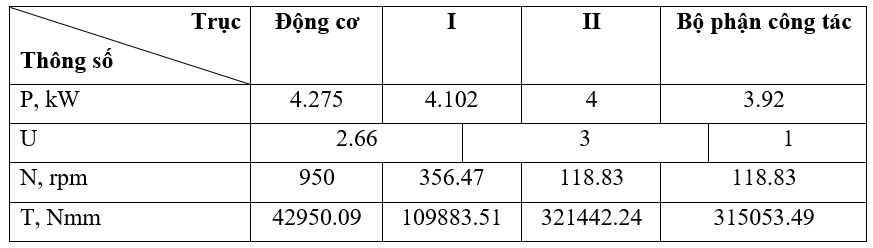
\includegraphics[width=1\textwidth]{pictures/bangdactinh.png}
    \caption{Bảng thông số hệ thống}
\end{figure}
    \chapter{Chọn bộ truyền đai}
\section{Chọn loại đai}
Dựa vào công suất động cơ là $P_{dc} = 4.275 \, \text{kW}$ và số vòng quay $n_{dc} = 1450$ vòng/phút \\
$\Rightarrow$ Chọn đai loại A \\    
\begin{table}[H]
\begin{tabular}{|c|c|c|c|c|c|c|c|}
    \hline 
    Ký hiệu đai & $b_p$  & $b_0$  & h  & $y_0$ (mm) & A ($mm^2$) & Chiều dài đai (m) & $d_{1min} (mm)$ \\ \hline
    A & 11 & 13 & 8 & 2.8 & 81 & 560 $\div$ 4000 & 90 \\ \hline
\end{tabular}
\caption{Thông số đai loại A}
\end{table}
\section{Tính đường kính bánh đai nhỏ}
\begin{equation}
    d_1 = 1.2d_{min} = 1.2 \cdot 90 = 108 \, \text{(mm)}
\end{equation}
Chọn theo dãy giá trị tiêu chuẩn, ta chọn $d_1 = 112 \, \text{(mm)}$.\\
Vận tốc dài trên bánh đai nhỏ:
\begin{equation}
    v_1 = \frac{\pi d_1 n_1}{60000} = \frac{\pi \cdot 112 \cdot 1450}{60000} = 8.503 \, \text{(m/s)}
\end{equation}
$\Rightarrow$ Thỏa điều kiện $v_1 < 25 \, \text{(m/s)}$ \\

\section{Chọn hệ số trượt tương đối và tính đường kính bánh đai lớn}
Chọn hệ số trượt tương đối $\xi = 0.01$. Từ công thức tỉ số của bộ truyền đai:
\begin{equation}
    u_d = \frac{d_2}{d_1 (1 - \xi)}
\end{equation}
\begin{equation}
    d_2 = u_d \cdot d_1 \cdot (1 - \xi) = 2.44 \cdot 112 \cdot (1 - 0.01) = 270.55 \, \text{(mm)}
\end{equation}
Chọn theo dãy giá trị tiêu chuẩn, ta chọn $d_2 = 280 \, \text{(mm)}$.\\
Tính lại tỷ số truyền:
\begin{equation}
    u_d = \frac{d_2}{d_1 (1 - \xi)} = \frac{280}{112 \cdot 0.99} = 2.52
\end{equation}
Để sai số tỷ số truyền bằng 0, ta tính lại đường kính bánh đai nhỏ:
\begin{equation}
    d_1 = \frac{d_2}{u_d \cdot (1 - \xi)} = \frac{280}{2.44 \cdot (1 - 0.01)} = 115.91 \, \text{(mm)}
\end{equation}

\section{Chọn khoảng cách trục $a$}
Theo các thông số $u_d = 2.44$ và $d_2 = 280 \, \text{mm}$:
\begin{equation}
    a = 1.2d_2 = 1.2 \cdot 280 = 336 \, \text{(mm)}
\end{equation}
Chiều dài đai:
\begin{equation}
    L = 2a + \pi \frac{d_1 + d_2}{2} + \frac{(d_2 - d_1)^2}{4a}
\end{equation}
\[
    L = 2 \cdot 336 + \pi \frac{115.91 + 280}{2} + \frac{(280 - 115.91)^2}{4 \cdot 336} = 1313.93 \, \text{(mm)}
\]
$\Rightarrow$ Chọn chiều dài đai $L = 1400 \, \text{mm}$ theo dãy giá trị tiêu chuẩn.\\
Tính lại khoảng cách trục:
\begin{equation}
    k = L - \pi \frac{d_1 + d_2}{2} = 1400 - \pi \frac{115.91 + 280}{2} = 778.106 \, \text{(mm)}
\end{equation}
\begin{equation}
    \Delta = \frac{d_2 - d_1}{2} = \frac{280 - 115.91}{2} = 82.045 \, \text{(mm)}
\end{equation}
\begin{equation}
    a = \frac{k + \sqrt{k^2 - 8\Delta^2}}{4} = \frac{778.106 + \sqrt{778.106^2 - 8 \cdot 82.045^2}}{4} = 380.2 \, \text{(mm)}
\end{equation}
Kiểm tra $a$ thỏa điều kiện:
\begin{equation}
    2(d_1 + d_2) \geq a \geq 0.7(d_1 + d_2)
\end{equation}
\[
    2(115.91 + 280) \geq a \geq 0.7(115.91 + 280)
\]
\[
    791.82 \geq a \geq 277.173
\]
$\Rightarrow a = 380.2 \, \text{(mm)}$ thỏa điều kiện. \\

\section{Tính toán vận tốc đai và số truyền đai}
Vận tốc dây đai:
\begin{equation}
    v = \frac{\pi d_1 n_1}{60000} = \frac{\pi \cdot 115.91 \cdot 1450}{60000} = 8.8 \, \text{(m/s)}
\end{equation}
Số vòng chạy đai trong 1 giây:
\begin{equation}
    i = \frac{v_1}{L} = \frac{8.8}{1400 \cdot 10^{-3}} = 6.286 \, \text{s}^{-1}
\end{equation}
$\Rightarrow$ Thỏa điều kiện $i \leq [i] = 10 \, \text{s}^{-1}$. \\

\section{Tính góc ôm đai bánh nhỏ}
\begin{equation}
    \alpha_1 = 180 - 57 \frac{d_2 - d_1}{a} = 180 - 57 \frac{280 - 115.91}{380.2} = 155.29^{\circ}
\end{equation}
\section{Các hệ số sử dụng}
Hệ số xét đến ảnh hưởng góc ôm đai:
\begin{equation}
    C_{\alpha} = 1.24(1 - e^{\frac{-\alpha_1}{110}}) = 1.24(1 - e^{\frac{-155.29}{110}}) = 0.938
\end{equation}

Hệ số xét đến ảnh hưởng vận tốc:
\begin{equation}
    C_v = 1 - 0.05(0.01v^2 - 1) = 1 - 0.05(0.01 \cdot 8.8^2 - 1) = 1.011
\end{equation}

Hệ số xét đến ảnh hưởng tỷ số truyền $u$:
\begin{equation}
    C_u = 1.14 \quad (v > 2.5 \, \text{m/s})
\end{equation}

Hệ số xét đến ảnh hưởng của chiều dài đai $L$:
\begin{equation}
    C_L = \sqrt[6]{\frac{L}{L_0}} = \sqrt[6]{\frac{1400}{1700}} = 0.968
\end{equation}

Hệ số xét đến sự ảnh hưởng của sự phân bố không đều tải trọng giữa các dây đai:
\begin{equation}
    C_z = 0.95 \quad \text{(chọn sơ bộ)}
\end{equation}

Hệ số xét đến ảnh hưởng của chế độ tải trọng:
\begin{equation}
    C_r = 0.9 \quad \text{(chọn sơ bộ)}
\end{equation}

Chọn công suất có ích cho phép theo GOST 1284.3 - 96, ta có: \\
Đai loại A, $d_1 = 115.91 \, \text{mm}$, $v_1 = 8.8 \, \text{m/s}$ \\
$\Rightarrow$ Chọn $[P_0] = 1.80$.

Tính số dây đai theo công thức:
\begin{equation}
    z \geq \frac{P_1}{[P_0] \cdot C_{\alpha} \cdot C_u \cdot C_L \cdot C_z \cdot C_r \cdot C_v} = \frac{4.102}{1.8 \cdot 0.938 \cdot 1.14 \cdot 0.968 \cdot 0.95 \cdot 0.9 \cdot 1.011} = 2.55
\end{equation}
$\Rightarrow$ Chọn $z = 3$ dây đai. \\
Kiểm nghiệm lại $C_z$: vì $z = 3$ nên $C_z = 0.95$ như đã chọn sơ bộ.

\section{Lực trên dây đai}
Tổng lực căng đai ban đầu trên cả dây đai:
\begin{equation}
    F_0 = z \cdot A \cdot [\sigma_0] = 3 \cdot 81 \cdot 1 = 243 \, \text{(N)}
\end{equation}
Trong đó: Đối với đai thang, $\sigma_0 \leq 1.5 \, \text{MPa}$ nên ta chọn $\sigma_0 = 1 \, \text{MPa}$, $z = 3$, $A = 81 \, \text{mm}^2$.

Lực căng trên mỗi dây đai:
\begin{equation}
    \frac{F_0}{z} = \frac{243}{3} = 81 \, \text{(N)}
\end{equation}

Tổng lực vòng có ích trên cả 3 đai:
\begin{equation}
    F_t = \frac{1000P_1}{v_1} = \frac{1000 \cdot 4.102}{8.8} = 466.136 \, \text{(N)}
\end{equation}

Lực vòng có ích trên mỗi dây đai:
\begin{equation}
    \frac{F_t}{z} = \frac{466.136}{3} = 155.379 \, \text{(N)}
\end{equation}

\section{Lực tác dụng lên trục}
\begin{equation}
    F_r \approx 2F_0\sin\left(\frac{\alpha_1}{2}\right) = 2 \cdot 243 \sin\left(\frac{155.29}{2}\right) = 474.744 \, \text{(N)}
\end{equation}

\section{Ứng suất lớn nhất trong dây đai}
\begin{equation}
    \sigma_{max} = \sigma_1 + \sigma_v + \sigma_{F1} = \sigma_0 + 0.5\sigma_t + \sigma_v + \sigma_{F1}
\end{equation}
\begin{equation}
    = \frac{F_0}{A} + 0.5 \cdot \frac{F_t}{A} + \rho \cdot v^2 \cdot 10^{-6} + E \cdot \frac{2 \cdot y_0}{d_1}
\end{equation}
\[
    = \frac{243}{3 \cdot 81} + 0.5 \cdot \frac{466.136}{3 \cdot 81} + 1000 \cdot 8.8^2 \cdot 10^{-6} + 60 \cdot \frac{2 \cdot 2.8}{115.19} = 4.88 \, \text{(MPa)}
\]

\section{Tuổi thọ dây đai}
\begin{equation}
    L_h = \frac{\left(\frac{\sigma_r}{\sigma_{max}}\right)^m \cdot 10^7}{2 \cdot 3600 \cdot i} = \frac{\left(\frac{9}{6.9}\right)^8 \cdot 10^7}{2 \cdot 3600 \cdot 6.286} = 29571.59 \, \text{(h)}
\end{equation}
Trong đó:
\begin{itemize}
    \item $\sigma_r = 9 \, \text{(MPa)}$ - giới hạn mỏi của đai thang.
    \item $m = 8$ - chỉ số mũ của đường cong mỏi đối với đai thang.
    \item $i = 6.286 \, \text{(s}^{-1}\text{)}$ - số vòng chạy của đai trong một giây.
\end{itemize}
\section{Bảng thông số bộ truyền đai}
\begin{table}[H]
    \centering
    \begin{tabular}{|l|c|}
        \hline
        \textbf{Thông số} & \textbf{Giá trị} \\ \hline
        Loại đai & A \\ \hline
        Đường kính bánh dẫn, $d_1$ (mm) & 115.91 \\ \hline
        Đường kính bánh bị dẫn, $d_2$ (mm) & 280 \\ \hline
        Chiều dài dây đai, $L$ (mm) & 1400 \\ \hline
        Khoảng cách trục, $a$ (mm) & 380.2 \\ \hline
        Góc ôm đai, $\alpha_1$ ($^\circ$) & 155.29 \\ \hline
        Số dây đai, $z$ & 3 \\ \hline
        Tuổi thọ đai, $L_h$ (h) & 29571.59 \\ \hline
    \end{tabular}
    \caption{Bảng thông số bộ truyền đai}
\end{table}
\cleardoublepage
    \section{Tính toán hộp giảm tốc bánh răng nghiêng 1 cấp}
\subsection{Chọn vật liệu cho bánh dẫn và bánh bị dẫn}
Hộp giảm tốc chịu công suất không quá lớn nên chỉ cần chọn vật liệu có độ cứng HB $\leq$ 350.
\begin{itemize}
    \item Bánh dẫn: thép c45 tôi cải thiện 	Bánh dẫn: thép c45 tôi cải thiện đạt độ rắn HB 230…280 có $\sigma_{b1} = 850MPa; \sigma_{ch1} = 650MPa; HB_1 = 250$
    \item o	Bánh bị dẫn: thép c45 tôi cải thiện đạt độ rắn HB 192…240 có $\sigma_{b2} = 750MPa; \sigma_{ch2} = 450MPa; HB_2 = 235$
\end{itemize}
\subsection{Số chu kỳ làm việc cơ sở}
\begin{center}
        $N_{HO_1} = 30.HB_1^{2,4} = 30.250^{2,4} = 1,71.10^7$ chu kỳ \\
        $N_{HO_2} = 30.HB_2^{2,4} = 30.235^{2,4} = 1,47.10^7$ chu kỳ \\
        $N_{FO_1} = N_{FO_2} = 5.10^6$ chu kỳ \\
\end{center}
\subsection{Số chu kỳ làm việc tương đương, xác định theo sơ đồ tải trọng}
\begin{center}
    $N_{HE_1} = 60.c.n.L_h = 60.1.482,5.14400 = 41,69.10{-7}$ chu kỳ
\end{center}
Với c = 1; n = 482,5 vòng/phút; $L_h$= 6.300.8 = 14400 giờ. 
\begin{center}
    $N_{HE_2} = \frac{N_{HE_1}}{\mu} = \frac{41,69.10^7}{6,3} = 6,617.10^7$ chu kỳ
\end{center}
Tương tự:
\begin{center}
    $N_{FE_1} = 60.c.n.L_h = 60.1.76,6.14400 = 6,618.10^{-7}$ chu kỳ
\end{center}
\begin{center}
    $N_{FE_2} = \frac{N_{FE_1}}{\mu} = \frac{41,69.10^7}{6,3} = 6,617.10^7$ chu kỳ
\end{center} 
Vì $N_{HE_1} > N_{HO_1}; N_{HE_2} > N_{HO_2}; N_{FE_1} > N_{FO_1}; N_{FE_2} > N_{FO_2}$ \\
$\Rightarrow K_{HL_1} = K_{HL_2} = K_{FL_1} = K_{FL_2} = 1$
\subsection{Giới hạn mỏi tiếp xúc và giới hạn mỏi uốn}
\[
    \sigma_{OH_{lim}} = 2HB + 70 
\]
\[
    \Rightarrow \sigma_{OH_{lim1}} = 2.250 + 70 = 570MPa
\]
\[
    \Rightarrow \sigma_{OH_{lim2}} = 2.235 + 70 = 540MPa
\]
\[
    \sigma_{OF_{lim}} = 1.8HB
\]
\[
    \Rightarrow \sigma_{OF_{lim1}} = 1.8.250 = 450MPa
\]
\[
    \Rightarrow \sigma_{OF_{lim2}} = 1.8.235 = 423MPa
\]
\subsection{Ứng suất tiếp xúc cho phép}
\[
    [\sigma_{H}] = \frac{\sigma_{OH_{lim}}.Z_R.Z_V.Z_L.Z_XH}{s_H}.K_{HL} = \frac{\sigma_{OH_{lim}}.0,9}{s_H}.K_{HL}
\]
Khi tôi cải thiện $s_H = 1,1$, do đó:
\[
    [\sigma_{H_1}] = \frac{570.0,9}{1,1}.1 = 466,37MPa
\]
\[
    [\sigma_{H_2}] = \frac{540.0,9}{1,1}.1 = 441,82MPa
\]
Ứng suất tính toán cho phép:
\[
    [\sigma_H] = 0,45.([\sigma_{H1}] + [\sigma_{H2}]) = 0,45.(466,37 + 441,82) = 408,68MPa
\]
Tuy nhiên
\[
    [\sigma_{min}] \leq [\sigma_H] \leq 1,25[\sigma_{min}] \Leftrightarrow 441.82 \leq [\sigma_H] \leq 552,275
\]
$\Rightarrow$ Ta chọn $[\sigma_H] = [\sigma_{H2}] = 441,82$ MPa
\subsection{Ứng suất uốn cho phép}
\[
    [\sigma_F] =\frac{\sigma_{OFlim}}{s_F}.K_{HL}
\]
Chọn $s_F = 1,75$, ta có: \\
\[
    [\sigma_{F1}] =\frac{\sigma_{OF1lim}}{s_F}.K_{HL} = \frac{450}{1,75}.1 = 257,143 (MPa)
\]
\[
    [\sigma_{F2}] =\frac{\sigma_{OF2lim}}{s_F}.K_{HL} = \frac{423}{1,75}.1 = 241,7 (MPa)
\]
\subsection{Khoảng cách trục}
Do bánh răng nằm đối xứng các ổ trục nên $\Psi_{ba} = 0,3 \div 0,5$, chọn $\Psi_{ba} = 0,4$ \\
Khi đó $\Psi_{bd} = \frac{\Psi_{ba}.(u+1)}{2} = \frac{0,4.(6,3+1)}{2} = 1,46$ \\
Từ đó tra theo bảng 6.4 ta chọn: $K_{H\beta} = 1,07$, $K_{F\beta} = 1,14$ \\
Tính khoảng cách trục: \\
\[
    a_w = 500.(u+1).\sqrt[3]{\frac{T_1.K_{H\beta}}{\Psi_{ba}.[\sigma_H]^2.u}} = 500.(6,3+1).\sqrt[3]{\frac{63,73.1,07}{0,4.408,68^2.6,3}} = 198,98 (mm)
\]
Theo tiêu chuẩn ta chọn $a_w = 200mm$
\subsection{Môđun răng}
\[
    m_n = (0,01 \div 0,02).a_w = 2 \div 4
\]
Theo tiêu chuẩn ta chọn $m_n = 4$
\subsection{Số răng}
Từ điều kiện $20^\circ \leq \beta \leq 8^\circ$ \\
\[
    \Leftrightarrow \frac{2.a_w.\cos8^\circ}{m_n.(u+1)} \leq z_1 \leq \frac{2.a_w.\cos20^\circ}{m_n.(u+1)}
\]
\[
    \Leftrightarrow \frac{2.200.\cos8^\circ}{4.(6,3+1)} \leq z_1 \leq \frac{2.200.\cos20^\circ}{4.(6,3+1)}
\]
\[
    \Leftrightarrow 13,56 \leq z_1 \leq 12,87
\]
$\Rightarrow$ Chọn $z_1 = 13 \Rightarrow z_2 = u.z_1 = 6,3.13 = 81,9$ \\
$\Rightarrow$ Chọn $z_2 = 82$ \\
Góc nghiêng răng: 
\[
    \beta = \arccos\frac{m_n.(z_1+z_2)}{2.a_w} = \arccos\frac{4.(13+82)}{2.200} = 18,2^\circ
\]
\subsection{Tỉ số truyền sau khi chọn răng}
\[
    u = \frac{z_2}{z_1} = \frac{82}{13} = 6,308
\]
\subsection{Các thông số hình học}
Đường kính vòng chia: \\
\[
    d_1 = \frac{m_n.z_1}{\cos\beta} = \frac{4.13}{\cos18,2^\circ} = 54,738 (mm)
\]
\[
    d_2 = \frac{m_n.z_2}{\cos\beta} = \frac{4.82}{\cos18,2^\circ} = 345,27 (mm)
\]
Đường kính vòng đỉnh: \\
\[
    d_{a1} = d_1 + 2.m_n = 54,738 + 2.4 = 62,738 (mm)
\]
\[
    d_{a2} = d_2 + 2.m_n = 354,27 + 2.4 = 362,27 (mm)
\]
Đường kính vòng đáy: \\ 
\[
    d_{f1} = d_1 - 2,5m_n = 62,738 - 2,5.4 = 44,738 (mm)
\]
\[
    d_{f2} = d_2 - 2,5m_n = 345,27 - 2,5.4 = 335,27 (mm)
\]
Tính lại khoảng cách trục: \\
\[
    a_w = \frac{m_n.(z_1+z_2)}{2\cos\beta} = \frac{4.(13+82)}{2.\cos18,2^\circ} = 200(mm)
\]
Chiều rộng vành răng: 
\begin{itemize}
    \item Bánh bị dẫn: $b_2 = \Psi_{ba}.a_w = 0,4.200 = 80(mm)$
    \item Bánh dẫn: $b_1 = b_2 + 5 = 85(mm)$
\end{itemize}
\subsection{Vận tốc vòng bánh răng}
\[
    v = \frac{\pi.d_1.n_1}{60000} = \frac{\pi.54,738.482,5}{60000} = 1,38 (m/s)
\]
Theo bảng 6.3 ta chọn cấp chính xác 9 với $v_{gh} = 6 m/s$
\subsection{Tính toán kiểm nghiệm giá trị ứng suất tiếp xúc}
Theo bảng 6.6 ta chọn hệ số tải trọng động $K_{HV} = 1,11$, $K_{FV} = 1,22$ \\
\[
    \sigma_H = \frac{z_M.z_H.z_\epsilon}{d_1}.\sqrt{\frac{2.T_1.10^3.K_{H\beta}.K_{HV}.(u+1)}{b_w.u}} 
\]
\[
    = \frac{190.2,3847.0,8124}{54,738}.\sqrt{\frac{2.63,73.10^3.1,07.1,11.(6,3+1)}{80.6,3}} = 314,887 (MPa)
\]
Với:
\begin{itemize}
    \item $Z_M = 190$ vì vật liệu bằng thép
    \item $Z_H = \sqrt{\frac{4.\cos\beta}{\sin(2.\alpha_{tw})}} = \sqrt{\frac{4.\cos18,2}{\sin(2.20,9637)}} = 2,3847$
    \item $\alpha_{tw} = \arctan(\frac{\tan\alpha_{nw}}{\cos\beta}) = \arctan(\frac{\tan20}{\cos18,2}) = 20,9637$
    \item $Z_\epsilon = \sqrt{\frac{1}{\epsilon_\alpha}} = \sqrt{\frac{1}{1,515}} = 0,8124$
    \item $\epsilon_\alpha = [1,88-3,2.(\frac{1}{z_1}+\frac{1}{z_2})].\cos\beta = [1,88-3,2.(\frac{1}{13}+\frac{1}{82})].\cos18,2 = 1,515$
\end{itemize}
\[
    \sigma_H = 314,887 MPa \leq 441,82 MPa
\]
    $\Rightarrow \sigma_H \leq [\sigma_H]$ thỏa mãn\\
\subsection{Số răng tương đương}
\[
    z_{v1} = \frac{z_1}{\cos^3(\beta)} = \frac{13}{\cos^3(18,2)} = 13,685 \Rightarrow z_{v1} = 14
\]
\[
    z_{v2} = \frac{z_2}{\cos^3(\beta)} = \frac{82}{\cos^3(18,2)} = 86,32 \Rightarrow z_{v1} = 87
\]
\subsection{Hệ số dạng răng}
\begin{itemize}
    \item Đối với bánh dẫn: $Y_{F1} = 3,47 + \frac{13,2}{z_{v1}} = 3,47 + \frac{13,2}{14} = 4,413$
    \item Đối với bánh bị dẫn: $Y_{F2} = 3,47 + \frac{13,2}{z_{v2}} = 3,47 + \frac{13,2}{87} = 3,622$
\end{itemize}
\subsection{Ứng suất uốn tính toán}
Đặc tính so sánh độ bền uốn:
\begin{itemize}
    \item Bánh dẫn: $\frac{[\sigma_{F1}]}{Y_{F1}} = \frac{257,143}{4,413} = 58,27$
    \item Bánh bị dẫn: $\frac{[\sigma_{F2}]}{Y_{F2}} = \frac{241,7}{3,622} = 66,73$
\end{itemize}
$\Rightarrow$ Ta kiểm tra độ bền uốn theo bánh dẫn có độ bền thấp hơn:\\
Ứng suất uốn tính toán:
\[
    \sigma_{F1} = \frac{Y_{F1}.F_t.K_{F1}.Y_\epsilon.Y_\beta}{b_2.m} = \frac{4,413.2328,547.1,39.0,66.0,6985}{80.4} = 20,577 (MPa)
\] 
Với: 
\begin{itemize}
    \item $Y_\epsilon = \frac{1}{\epsilon_\alpha} = \frac{1}{1,515} = 0,66$
    \item $F_t = 2.10^3.\frac{T_1}{d_{w1}} = 2.10^3.\frac{63,73}{54,738} = 2328,547$
    \item $Y_\beta = 1 - \epsilon_\beta\frac{\beta}{120} = 1 - 1,988\frac{18,2}{120} = 0,6985$
    \item $\epsilon_\beta = b_w.\frac{\sin\beta}{\pi.m} = 80.\frac{\sin18,2}{\pi.4} = 1,988$
    \item $K_{F1} = K_{F\alpha}.K_{F\beta}.K_{FV} = 1.1,14.1,22 = 1,39$
    \item $K_{F\alpha} = \frac{4 + (\epsilon_\alpha - 1).(n_{cx} - 5)}{4\epsilon_\alpha} = \frac{4 + (1,515 - 1).(9 - 5)}{4.1,515} = 1$
\end{itemize}
$\Rightarrow \sigma_{F1} < [\sigma_{F1}] = 257,143$ MPa do đó độ bền uốn thỏa\\
\subsection{Phân tích lực}
\begin{figure}[H]
    \centering
    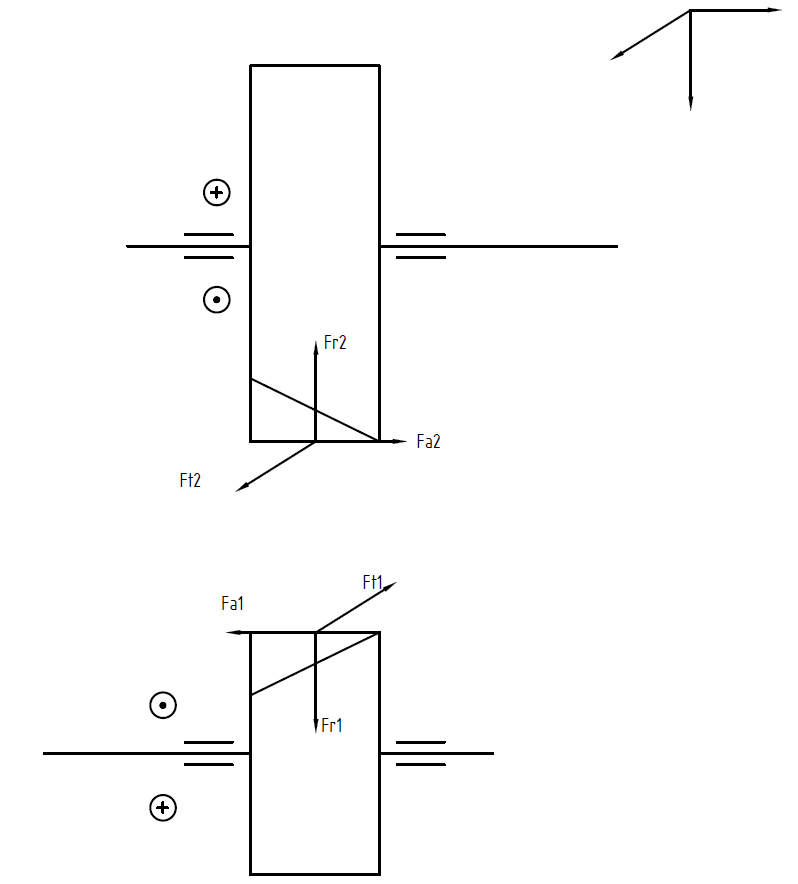
\includegraphics[width=0.5\textwidth]{pictures/phantichluc.png}
\end{figure}
\cleardoublepage
    % \section{Thiết kế trục I}
\subsection{Chọn vật liệu}
Chọn vật liệu chế tạo là thép $C_{45}$, giới hạn bền $\sigma_b =736MPa$, giới hạn chảy $\sigma_{ch} = 490MPa$.
Ứng suất uốn cho phép $[\sigma_F] = 48MPa$, ứng suất tiếp cho phép $[\tau] = 22MPa$.
\subsection{Phân tích lực trên trục}
\begin{itemize}
    \item Lực tác dụng lên trục của bộ truyền đai: $F_r = 833,8N$
    \item Lực vòng bánh dẫn: $F_{t1} = 2.10^3\frac{T_1}{d_1} = 2.10^3.\frac{63,73}{54,738} = 2328,55N$
    \item Lực hướng tâm trên bánh dẫn: $F_{r1} = \frac{F_{t1}.\tan\alpha}{\cos\beta} = \frac{2328,55.\tan20}{\cos18,2} = 892,1544N$
    \item Lực dọc trục trên banh dẫn: $F_{a1} = F_{t1}.\tan\beta = 2328,55.\tan18,2 = 765,588N$
\end{itemize}

\subsection{Thiết kế sơ bộ kết cấu trục}
Tính sơ bộ đường kính trục: \\
\[
    d_1 = 10\sqrt[3]{\frac{16T_1}{\pi[\tau]}} = 10\sqrt[3]{\frac{16.63,73}{\pi.22}} = 24,526(mm)
\]
$\Rightarrow$ Chọn d = 25mm theo tiêu chuẩn. \\
Khoảng cách giữa các ổ trong hộp giảm tốc bánh răng trụ một cấp: \\
\[
    l \approx l_1 + 2x + w = 85 + 2.10 + 35 = 140(mm)
\]
Trong đó: 
\begin{itemize}
    \item $l_1 = b_1 = 85(mm)$ - Kết quả tính bộ truyền bánh răng
    \item $w = 35(mm) - w = 30 \div 55(mm)$ khi $T = 60 \div 80(Nm)$
    \item $x = 10(mm)$ - Khe hở giữa bánh răng và thành trong hộp giảm tốc
\end{itemize}
Khoảng cách f theo bảng 10.3 không nhỏ hơn $55 \div 75$ nên ta chọn $f = 60mm.$
\subsection{Vẽ biểu đồ momen uốn và xoắn}
Trong mặt phẳng đứng zy, phương trình cân bằng momen: $M_{A} = 0$ \\
Suy ra:
\[
    F_r .0,06 - F_{r1}.0,07 + M_{a1} + R_{BY}.0,14 = 0
\]
Trong đó $M_{a1} = \frac{F_{a1}.d_1.10^{-3}}{2} = \frac{765,588.54,738.10^{-3}}{2} = 20,95Nm$ \\
\begin{equation}
    \Leftrightarrow 833,8.0,06 - 892,1544.0,07 + 20,95 + R_{BY}.0,14 = 0
\end{equation}
Phương trình cân bằng lực theo trục y: \\
\[
    -F_r + R_{AY} + -F_{r1} + R_{BY} = 0
\]
\begin{equation}
    \Leftrightarrow -833,8 + R_{AY} - 892,1544 + R_{BY} = 0
\end{equation}
Từ (1) và (2) ta giải hệ phương trình tìm được $R_{AY} = 1786,86N$ và $R_{BY} = -60,9N$. \\
Trong mặt phẳng nằm ngang zx, vì lực $F_{t1}$ nằm đối xứng với hai ổ, nên: 
\[
    R_{AX} = R_{BX} = \frac{F_{t1}}{2} = \frac{2328,55}{2} = 1164,27N
\]
Vẽ biểu đồ momen với:
\begin{itemize}
    \item $M_{XD} = R_{BY}.0,07 = 4,263Nm$
    \item $M_{XA} = F_r.0,06 = 50,028Nm$
    \item $M_{YD} = R_{BX}.0,07 = 81,5Nm$
\end{itemize}   
Momen xoắn T1 = 63,73Nm. \\
\begin{figure}[H]
    \centering
    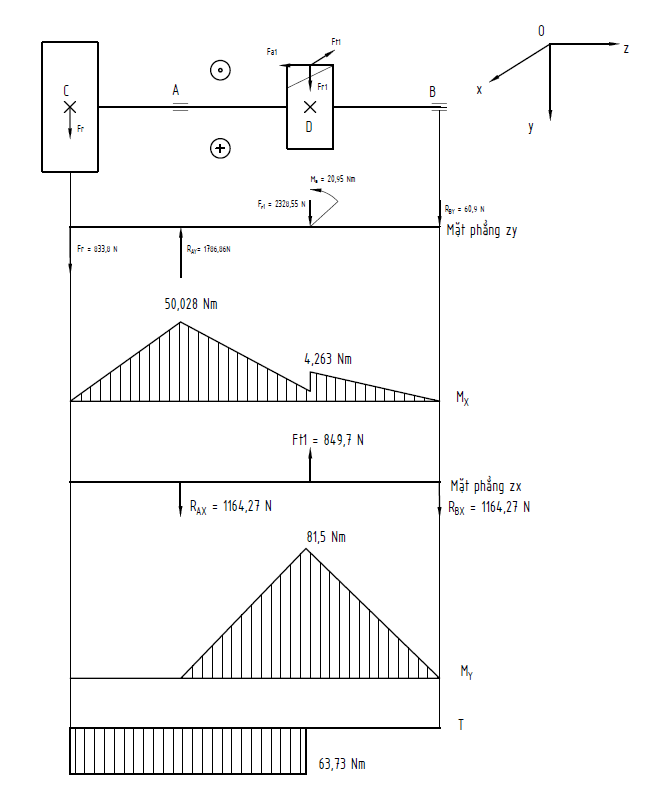
\includegraphics[width=1.1\textwidth]{pictures/luctruc1.png}
\end{figure}
\subsection{Momen uốn và momen xoắn tại vị trí nguy hiểm}
Các biểu đồ momen cho thấy tiết diện nguy hiểm nhất tại vị trí D. \\
Momen uốn tại D: 
\[
    M_D = \sqrt{M_{XD}^2 + M_{YD}^2} = \sqrt{4,263^2 + 81,5^2} = 81,61Nm
\]
Momen xoắn tại D: $T = 63,73Nm$ \\
Momen tương đương tại D: \\
$M_{td} = \sqrt{M_{XD}^2 + M_{YD}^2 + 0,75T^2} = \sqrt{4,263^2 + 81,5^2 + 0,75.63,73^2} = 98,52 Nm$\\
\[
d = \sqrt[3]{\frac{M_{td}.10^3}{0,1.[\sigma]}} = 27,38 mm
\]
Tại vị trí D có lắp bánh răng nên cần tăng đường kính trục thêm 5\% nên chọn d = 30mm. 
\subsection{Ứng suất pháp tại tiết diện D}
Ta bỏ qua ảnh hưởng của lực dọc trục nên ứng suất pháp tại tiết diện này thay đổi theo
chu kỳ đối xứng biên độ:
\[  
    \sigma_a = \sigma_F = \frac{M_D.10^3}{W}
\]
Tại vị trí D trục có một then, với đường kính d = 30mm, ta chọn then có chiều rộng $b = 8mm$, chiều cao $h = 7mm$, chiều sâu rãnh then trên trục t = 4mm, chiều sâu rãnh then trên mayơ $t_1 = 3,8 mm$. Khi đó: 
\[
    W = \frac{\pi d^3}{32} - \frac{bt(d-t)^2}{2d} = \frac{\pi 25^3}{32} - \frac{8.4(25-4)^2}{2.25} = 1251,741mm^3
\]
Do đó:  
\[
    \sigma_a = \frac{98,52.10^3}{1251,741} = 78,706MPa
\]
\begin{figure}[H]
    \centering
    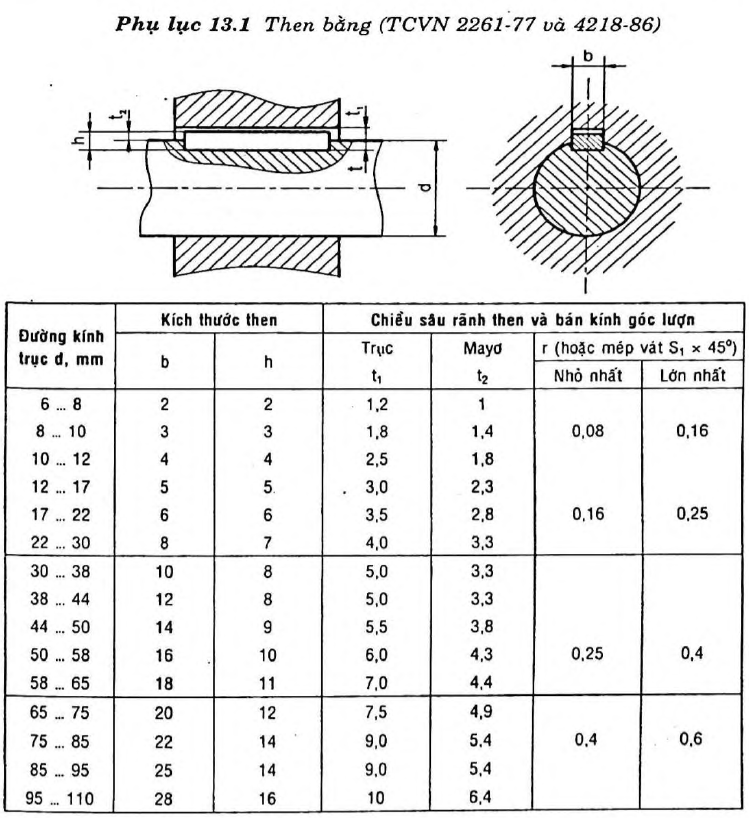
\includegraphics[width=0.8\textwidth]{pictures/then.png}
    \caption{Tiêu chuẩn chọn then}
\end{figure}
\subsection{Kiểm nghiệm then tại vị trí gắn bánh răng D}
\begin{figure}[H]
    \centering
    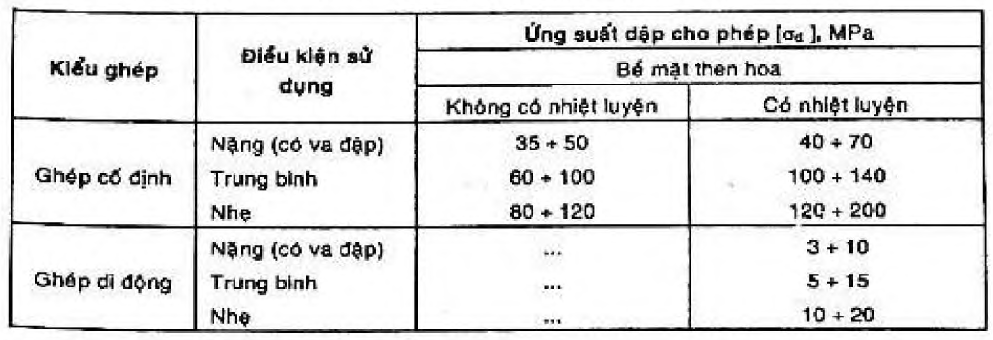
\includegraphics[width=0.8\textwidth]{pictures/then1.png}
    \caption{Trị số ứng xuất dập cho phép của then hoa}
\end{figure}
Chọn chiều dài l của then theo tiêu chuẩn l = 56mm.\\
Chọn ứng suất dập cho phép $[\sigma_d]$ = 150MPa theo bảng 16.1. \\
Chọn ứng suất cắt cho phép $[\tau_d]$ = 90MPa \\
Kiểm tra độ bền dập theo công thức:
\[
    \sigma_d = \frac{F}{t_2l_l} = \frac{2T.10^3}{t_2dl_l} = \frac{2.63,73.10^3}{2,8.25.48} = 37,9MPa < [\sigma_d] = 150MPa
\]
Trong đó:
\begin{itemize}
    \item $l_l = l - b = 56 - 8 = 48mm$
    \item $h = 7mm$
    \item $t_2 = 0,4h = 2,8mm$
\end{itemize}
Kiểm tra then theo độ bền cắt: 
\[
    \tau_d = \frac{T}{bl_l} = \frac{2T.10^3}{bdl_l} = \frac{2.63,73.10^3}{8.25.48} = 13,28MPa < [\tau_d] = 90MPa 
\]
$\Rightarrow$ Vậy then này đạt độ bền tính toán.
\subsection{Ứng suất xoắn tại vị trí D}
\[
    \tau = \frac{T_1.10^3}{W_o} = \frac{63,73.10^3}{2785,7216} = 22,88MPa
\]
Trong đó momen cản xoắn:
\[
    W_o = \frac{\pi d^3}{16} - \frac{bt(d-t)^2}{2d} = \frac{\pi 25^3}{16} - \frac{8.4(25-4)^2}{2.25} = 2785,7216mm^3
\]
Khi ứng suất xoắn thay đổi theo chu kỳ mạch động: 
\[
    \tau_\alpha = \sigma_m = \frac{\sigma}{2} = \frac{22,88}{2} = 11,44MPa
\]
\subsection{Xác định hệ số an toàn tại vị trí D}
Tại tiết diện D có sự tập trung ứng suất là rãnh then. Theo bảng 10.9 ta chọn $K_\sigma =2,05$, $K_\tau = 1,9$ với $\sigma_b = 736MPa < 800MPa$ \\
Theo bảng 10.4 với d = 30mm ta chọn $\epsilon_\sigma = 0,91$ và $\epsilon_\tau = 0.89$ \\
Hệ số $\Psi_\sigma = 0,035$ và $\Psi_\tau = 0,07$ \\ 
Với hệ số tăng bền bề mặt, chọn phương pháp phun bi nên $\beta = 1,7$. \\
Với thép C45, d =25mm chọn giới hạn mỏi của vật liệu $\sigma_{-1} = 432MPa$, $\tau_{-1} = 255MPa$. \\
Xác định hệ số an toàn tại D theo công thức:
\[
    s_\sigma = \frac{\sigma_{-1}}{K_\sigma \sigma_a / \epsilon_\sigma \beta + \Psi_\sigma \sigma_m} = \frac{432}{2,05.66,47/0,91.1,7 + 0,035.0} = 4,9
\]
\[
    s_\tau = \frac{\tau_{-1}}{K_\tau \tau_a / \epsilon_\tau \beta + \Psi_\tau \tau_m} = \frac{255}{2,05.11,44/0,89.1,7 + 0,07.11,44} = 15,943
\]
Hệ số an toàn:
\[
    s = \frac{s_\sigma s_\tau}{\sqrt{s_\sigma^2 + s_\tau^2}} = \frac{4,9.15,943}{\sqrt{4,9^2 + 15,943^2}} = 4,684 > [s] = 1,5
\]
Do đó điều kiện bền mỏi của trục tại tiết diện D được thỏa.
\subsection{Ứng suất pháp tại tiết diện C}
Ta bỏ qua ảnh hưởng của lực dọc trục nên ứng suất pháp tại tiết diện này thay đổi theo chu kỳ đối xứng biên độ:
\[
    \sigma_a = \sigma_F = \frac{M_C.10^3}{W}
\]
Trong đó $M_C = \sqrt{M_{CX}^2 + M_{CY}^2 + 0,75T^2} = 55,19 Nm$\\
Tại vị trí C trục có một then, với đường kính d = 30mm, ta chọn then có chiều rộng $b = 8mm$, chiều cao $h = 7mm$, chiều sâu rãnh then trên trục t = 4mm, chiều sâu rãnh then trên mayơ $t_1 = 3,8 mm$. Khi đó: 
\[
    W = \frac{\pi d^3}{32} - \frac{bt(d-t)^2}{2d} = \frac{\pi 25^3}{32} - \frac{8.4(25-4)^2}{2.25} = 1251,741mm^3
\]
Do đó:  
\[
    \sigma_a = \frac{55,19.10^3}{1251,741} = 44,09MPa
\]
\subsection{Kiểm nghiệm then tại vị trí gắn bánh đai C}
Chọn chiều dài l của then theo tiêu chuẩn l = 56mm.\\
Chọn ứng suất dập cho phép $[\sigma_d]$ = 150MPa theo bảng 16.1. \\
Chọn ứng suất cắt cho phép $[\tau_d]$ = 90MPa \\
Kiểm tra độ bền dập theo công thức:
\[
    \sigma_d = \frac{F}{t_2l_l} = \frac{2T.10^3}{t_2dl_l} = \frac{2.63,73.10^3}{2,8.25.48} = 37,9MPa < [\sigma_d] = 150MPa
\]
Trong đó:
\begin{itemize}
    \item $l_l = l - b = 56 - 8 = 48mm$
    \item $h = 7mm$
    \item $t_2 = 0,4h = 2,8mm$
\end{itemize}
Kiểm tra then theo độ bền cắt: 
\[
    \tau_d = \frac{T}{bl_l} = \frac{2T.10^3}{bdl_l} = \frac{2.63,73.10^3}{8.25.48} = 13,28MPa < [\tau_d] = 90MPa 
\]
$\Rightarrow$ Vậy then này đạt độ bền tính toán.
\subsection{Ứng suất xoắn tại vị trí C}
\[
    \tau = \frac{T_1.10^3}{W_o} = \frac{63,73.10^3}{2785,7216} = 22,88MPa
\]
Trong đó momen cản xoắn:
\[
    W_o = \frac{\pi d^3}{16} - \frac{bt(d-t)^2}{2d} = \frac{\pi 25^3}{16} - \frac{8.4(25-4)^2}{2.25} = 2785,7216mm^3
\]
Khi ứng suất xoắn thay đổi theo chu kỳ mạch động: 
\[
    \tau_\alpha = \sigma_m = \frac{\sigma}{2} = \frac{22,88}{2} = 11,44MPa
\]
\subsection{Xác định hệ số an toàn tại vị trí C}
Tại tiết diện D có sự tập trung ứng suất là rãnh then. Theo bảng 10.9 ta chọn $K_\sigma =2,05$, $K_\tau = 1,9$ với $\sigma_b = 736MPa < 800MPa$ \\
Theo bảng 10.4 với d = 30mm ta chọn $\epsilon_\sigma = 0,91$ và $\epsilon_\tau = 0.89$ \\
Hệ số $\Psi_\sigma = 0,035$ và $\Psi_\tau = 0,07$ \\ 
Với hệ số tăng bền bề mặt, chọn phương pháp phun bi nên $\beta = 1,7$. \\
Với thép C45, d =30mm chọn giới hạn mỏi của vật liệu $\sigma_{-1} = 432MPa$, $\tau_{-1} = 255MPa$. \\
Xác định hệ số an toàn tại D theo công thức:
\[
    s_\sigma = \frac{\sigma_{-1}}{K_\sigma \sigma_a / \epsilon_\sigma \beta + \Psi_\sigma \sigma_m} = \frac{432}{2,05.40,09/0,91.1,7 + 0,035.0} = 8,13
\]
\[
    s_\tau = \frac{\tau_{-1}}{K_\tau \tau_a / \epsilon_\tau \beta + \Psi_\tau \tau_m} = \frac{255}{2,05.11,44/0,89.1,7 + 0,07.11,44} = 15,943
\]
Hệ số an toàn:
\[
    s = \frac{s_\sigma s_\tau}{\sqrt{s_\sigma^2 + s_\tau^2}} = \frac{8,13.15,943}{\sqrt{8,13^2 + 15,943^2}} = 7,24 > [s] = 1,5
\]
Do đó điều kiện bền mỏi của trục tại tiết diện C được thỏa.
    % \section{Tính toán trục 2}
\subsection{Chọn vật liệu}
Chọn vật liệu chế tạo là thép $C_{45}$, giới hạn bền $\sigma_b =736MPa$, giới hạn chảy $\sigma_{ch} = 490MPa$.
Ứng suất uốn cho phép $[\sigma_F] = 48MPa$, ứng suất tiếp cho phép $[\tau] = 22MPa$.
\subsection{Phân tích lực trên trục}
\begin{itemize}
    \item Lực vòng bánh dẫn: $F_{t2} = F_{t1} = 2328,55N$
    \item Lực hướng tâm trên bánh bị dẫn: $F_{r2} = F_{r1} = 892,1544N$
    \item Lực dọc trục trên banh dẫn: $F_{a2} = F_{a2} = 765,588N$
    \item Lực nối trục: $F_{rk} \approx 0,2.F_{t} = 1285N$ \\
    Trong đó $F_t = \frac{2T_{II}}{D} = \frac{2.385,5}{120.10^-3} = 6425N$
\end{itemize}
\subsection{Thiết kế sơ bộ kết cấu trục}
Tính sơ bộ đường kính trục: \\
\[
    d_2 = 10\sqrt[3]{\frac{16T_2}{\pi[\tau]}} = 10\sqrt[3]{\frac{16.385,5}{\pi.22}} = 44,69(mm)
\]
$\Rightarrow$ Chọn d = 45mm theo tiêu chuẩn. \\
Khoảng cách giữa các ổ trong hộp giảm tốc bánh răng trụ một cấp: \\
\[
    l \approx l_2 + 2x + w = 85 + 2.10 + 35 = 140(mm)
\]
Trong đó: 
\begin{itemize}
    \item $l_2 = 85(mm)$ - Kết quả tính bộ truyền bánh răng
    \item $w = 35(mm) - w = 40 \div 80(mm)$ khi $T = 200 \div 400(Nm)$
    \item $x = 10(mm)$ - Khe hở giữa bánh răng và thành trong hộp giảm tốc
\end{itemize}
Khoảng cách f theo bảng 10.3 không nhỏ hơn $70 \div 105$ nên ta chọn $f = 90mm.$
\subsection{Vẽ biểu đồ momen uốn và xoắn}
Trong mặt phẳng đứng zy, phương trình cân bằng momen: $M_{A} = 0$. Suy ra:
\[
    F_{r2}.85.10^{-3} + M_{a2} + R_{BY}.140.10^{-3} = 0
\]
Trong đó $M_{a2} = \frac{F_{a2}.d_2.10^{-3}}{2} = \frac{279,367.345,27.10^{-3}}{2} = 48,23Nm$ \\
\begin{equation}
    \Leftrightarrow 892,1544.85.10^{-3} + 48,23 + R_{BY}.140.10^{-3} = 0
\end{equation}
Phương trình cân bằng lực theo trục y: \\
\[
    R_{AY}  + R_{BY} + F_{r2} = 0
\]
\begin{equation}
    \Leftrightarrow R_{AY} + R_{BY} + 892,1544 = 0
\end{equation}
Từ (3) và (4) ta giải hệ phương trình tìm được $R_{AY} = -6N$ và $R_{BY} = -886,165N$. \\
Trong mặt phẳng đứng zx, phương trình cân bằng momen: $M_{A} = 0$. Suy ra:
\[
    -F_{t2}.85.10^{-3} - F_{rk}.260.10^{-3} + R_{BX}.140.10^-3 = 0
\]
\begin{equation}
    \Leftrightarrow -2328,55.85.10^{-3} - 465,71.260.10^{-3} + R_{BX}.140.10^{-3} = 0
\end{equation}
Phương trình cân bằng lực theo trục y: \\
\[
    R_{AX} + R_{BX} - F_{t2} - F_{rk}= 0
\]
\begin{equation}
    \Leftrightarrow R_{AX} + R_{BX} - 2328,55 - 1285 = 0
\end{equation}
Từ (3) và (4) ta giải hệ phương trình tìm được $R_{AX} = 1334,9N$ và $R_{BX} = 2278,6525N$. \\
Vẽ biểu đồ momen với:
\begin{itemize}
    \item $M_{XC_1} = R_{AY}.0,085 = 0,51Nm$
    \item $M_{XC_2} = -M_{XC_1} + M_{a2} = 48,74Nm$
    \item $M_{XB} = M_{XC_2} + R_{BY}.0,085 = 0Nm$
    \item $M_{YC} = R_{AX}.0,085 = 113,4665Nm$
    \item $M_{YB} = - M_{YC} + 1285.0,085 = -4,24Nm$
\end{itemize}
Momen xoắn T2 = 385,5Nm. \\
\begin{figure}[H]
    \centering
    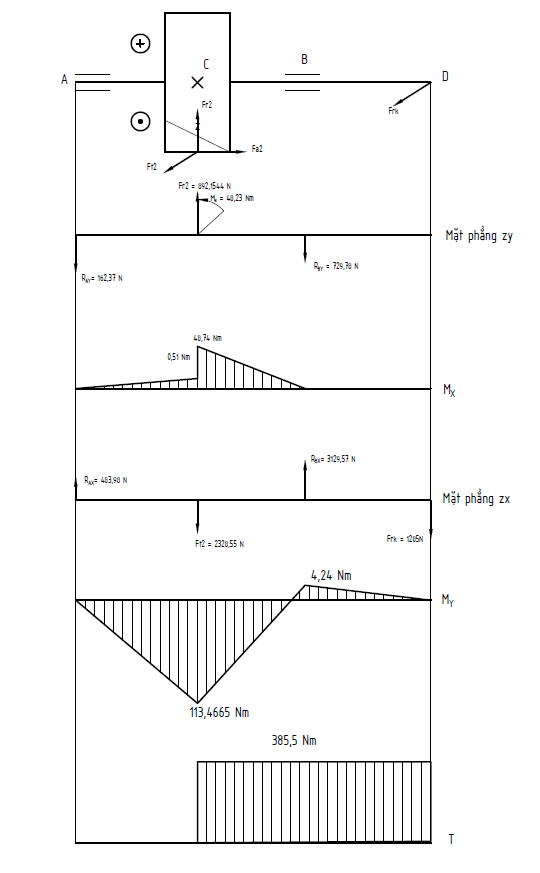
\includegraphics[width=1\textwidth]{pictures/luctruc2.png}
\end{figure}
Các biểu đồ momen cho thấy tiết diện nguy hiểm nhất tại vị trí C. \\
Momen uốn tại B:
\[
    M_B = \sqrt{M_{XC}^2 + M_{YC}^2} = \sqrt{48,74^2 + 113,4665^2} = 123,49Nm
\]
Momen xoắn tại B: $T = 385,5Nm$ \\
Momen tương đương tại C:
\[
    M_{td} = \sqrt{M_{XC}^2 + M_{YC}^2 + 0,75T^2} = \sqrt{48,74^2 + 113,4665^2 + 0,75.385,5^2} = 353,96Nm
\]
\[
d = \sqrt[3]{\frac{M_{td}.10^3}{0,1.[\sigma]}} = 41,9 mm
\]
Tại vị trí B có lắp bánh răng nên cần tăng đường kính trục thêm 5\% nên chọn d = 45mm.
\subsection{Ứng suất pháp tại tiết diện B}
Ta bỏ qua ảnh hưởng của lực dọc trục nên ứng suất pháp tại tiết diện này thay đổi theo
chu kỳ đối xứng biên độ:
\[  
    \sigma_a = \sigma_F = \frac{M_B.10^3}{W}
\]
Trục có một then, với đường kính d = 45mm, ta chọn then có chiều rộng b = 14mm, chiều cao h = 9mm, chiều sâu rãnh then trên trục t = 5,5mm, chiều sâu rãnh then trên mayơ $t_1 = 3,8 mm$. Khi đó: 
\[
    W = \frac{\pi d^3}{32} - \frac{bt(d-t)^2}{2d} = \frac{\pi 45^3}{32} - \frac{14.5,5(45-5,5)^2}{2.45} = 7516mm^3
\]
Do đó: 
\[
    \sigma_a = \frac{115,65.10^3}{7516} = 15,39MPa
\]
\subsection{Kiểm nghiệm then}
Chọn chiều dài l của then theo tiêu chuẩn l = 70mm.\\
Chọn ứng suất dập cho phép $[\sigma_d]$ = 150MPa theo bảng 16.1. \\
Chọn ứng suất cắt cho phép $[\tau_d]$ = 90MPa \\
Kiểm tra độ bền dập theo công thức:
\[
    \sigma_d = \frac{F}{t_2l_l} = \frac{2T.10^3}{t_2dl_l} = \frac{2.385,5.10^3}{3,6.45.56} = 85MPa < [\sigma_d] = 150MPa
\]
Trong đó:
\begin{itemize}
    \item $l_l = l - b = 70 - 14 = 56mm$
    \item $h = 9mm$
    \item $t_2 = 0,4h = 3,6mm$
\end{itemize}
Kiểm tra then theo độ bền cắt: 
\[
    \tau_d = \frac{T}{bl_l} = \frac{2T.10^3}{bdl_l} = \frac{2.385,5.10^3}{14.45.56} = 21,85MPa < [\tau_d] = 90MPa 
\]
$\Rightarrow$ Vậy then này đạt độ bền tính toán.
\subsection{Ứng suất xoắn}
\[
    \tau = \frac{T_2.10^3}{W_o} = \frac{385,5.10^3}{16557,5} = 23,28MPa
\]
Trong đó momen cản xoắn:
\[
    W = \frac{\pi d^3}{16} - \frac{bt(d-t)^2}{2d} = \frac{\pi 45^3}{16} - \frac{14.5,5(45-5,5)^2}{2.45} = 16557,5mm^3
\]
Khi ứng suất xoắn thay đổi theo chu kỳ mạch động: 
\[
    \tau_\alpha = \sigma_m = \frac{\sigma}{2} = \frac{23,28}{2} = 11,64MPa
\]
\subsection{Xác định hệ số an toàn}
Tại tiết diện B có sự tập trung ứng suất là rãnh then. Theo bảng 10.9 ta chọn $K_\sigma =2,05$, $K_\tau = 1,9$ với $\sigma_b = 736MPa < 800MPa$ \\
Theo bảng 10.4 với d = 45mm ta chọn $\epsilon_\sigma = 0,84$ và $\epsilon_\tau = 0.78$ \\
Hệ số $\Psi_\sigma = 0,035$ và $\Psi_\tau = 0,07$ \\ 
Với hệ số tăng bền bề mặt, chọn phương pháp phun bi nên $\beta = 1,7$. \\
Với thép C45, d =45mm chọn giới hạn mỏi của vật liệu $\sigma_{-1} = 383MPa$, $\tau_{-1} = 226MPa$. \\
Xác định hệ số an toàn tại D theo công thức:
\[
    s_\sigma = \frac{\sigma_{-1}}{K_\sigma \sigma_a / \epsilon_\sigma \beta + \Psi_\sigma \sigma_m} = \frac{383}{2,05.15,39/0,84.1,7 + 0,035.0} = 17,335
\]
\[
    s_\tau = \frac{\tau_{-1}}{K_\tau \tau_a / \epsilon_\tau \beta + \Psi_\tau \tau_m} = \frac{226}{2,05.11,64/0,78.1,7 + 0,07.11,64} = 12,015
\]
Hệ số an toàn:
\[
    s = \frac{s_\sigma s_\tau}{\sqrt{s_\sigma^2 + s_\tau^2}} = \frac{17,335.12,015}{\sqrt{17,335^2 + 12,015^2}} = 9,875 > [s] = 1,5
\]
Do đó điều kiện bền mỏi của trục tại tiết diện B được thỏa.
\cleardoublepage
    % \section{Chọn ổ lăn trục 1}
\subsection{Chọn trước ổ}
\begin{figure}[H]
    \centering
    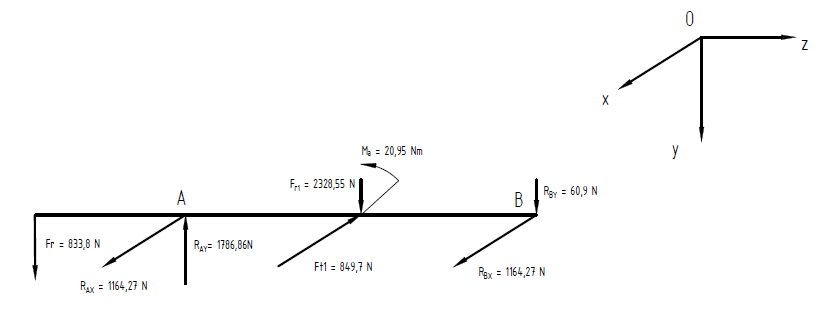
\includegraphics[width=1\textwidth]{pictures/tinholan1.png}
\end{figure}
Xác định phản lực tại các vị trí A và B:
\[
    F_{rA} = \sqrt{R_{AX}^2 + R_{AY}^2} = \sqrt{1164,27^2 + 1786,86^2} = 2132,7N
\]
\[
    F_{rB} = \sqrt{R_{BX}^2 + R_{BY}^2} = \sqrt{1164,27^2 + 60,9^2} = 1165,86N
\]
Tại vị trí A có lực tập trung lớn hơn nên ta chọn ổ lăn theo vị trí A của trục I.
\[
    \frac{F_a}{F_r} = \frac{765,588}{2132,7} = 0,359
\]
Vì $0,3 < \frac{F_a}{F_r} = 0,36 < 0,7$ nên ta chọn loại ổ bi đỡ là ổ bi đỡ chặn 1 dãy. \\
Ta có đường kính trục tại ổ lăn: d = 25mm \\
$\Rightarrow$ Chọn ổ lăn loại ổ bi đỡ chặn, cỡ trung có ký hiệu 46305 với $C = 21100N$ và $C_o = 14900N$.
\begin{figure}[H]
    \centering
    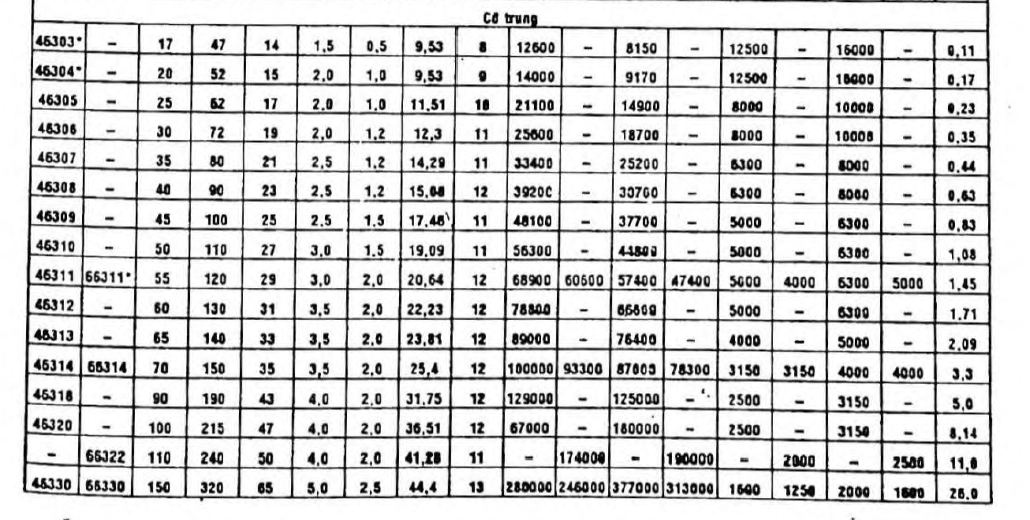
\includegraphics[width=1\textwidth]{pictures/chono1.png}
    \caption{Tiêu chuẩn chọn ổ đỡ chặn cỡ trung}
\end{figure}
\subsection{Tính ổ lăn theo khả năng tải trọng}
\subsubsection*{Chọn các hệ số}
\begin{itemize}
    \item Chọn hệ số $K_\alpha = 1$ do tải trọng tĩnh.
    \item Chọn hệ số $K_t = 1$ do làm việc ở nhiệt độ thường.
    \item Chọn hệ số $V = 1$ do vòng trong quay.\\
    Chọn hệ số X và Y: \\
    $\frac{F_a}{C_o} = \frac{765,588}{14900} = 0,0514 \Rightarrow$ chọn e = 0,34.\\
    $\frac{F_a}{VF_r} = \frac{765,588}{1.2132,7} = 0,359 > e = 0,34$ nên chọn X = 0,45 và Y = 1,62.
\end{itemize}
\subsubsection*{Thời gian làm việc tính bằng triệu vòng quay}
\[
    L = \frac{60L_hn}{10^6} = \frac{60.6.280.8.2.482,5}{10^6} = 778,176 
\]
\cleardoublepage
\subsubsection*{Tải trọng quy ước tác dụng lên ổ lăn}
\[
    Q = (XVF_r+YF_\alpha)K_\sigma K_\tau = (0,45.1.2132,7 + 1,62.765,588).1.1 = 2200N
\]
\[
    C_t = Q\sqrt[m]{L} =2200\sqrt[3]{778,176} = 2200.11,5 = 20235,6N
\]
Vì $C_t < C = 21100N$ nên việc chọn cỡ nhẹ là hợp lý.
\begin{center}
\begin{tabular}{|c|c|c|c|c|c|c|c|}
    \hline
       \textbf{Ký hiệu} & \textbf{d, mm} & \textbf{D, mm} & \textbf{B, Nm} & \textbf{r, mm} & \textbf{C, N} & \textbf{$C_o$, N} & \textbf{$L_h$, giờ} \\
    \hline
    46305 & 25 & 52 & 17 & 2 & 21100 & 14900 & 26880 \\
    \hline
\end{tabular}
\end{center}
\section{Chọn ổ lăn trục 2}
\subsection{Chọn trước ổ}
\begin{figure}[H]
    \centering
    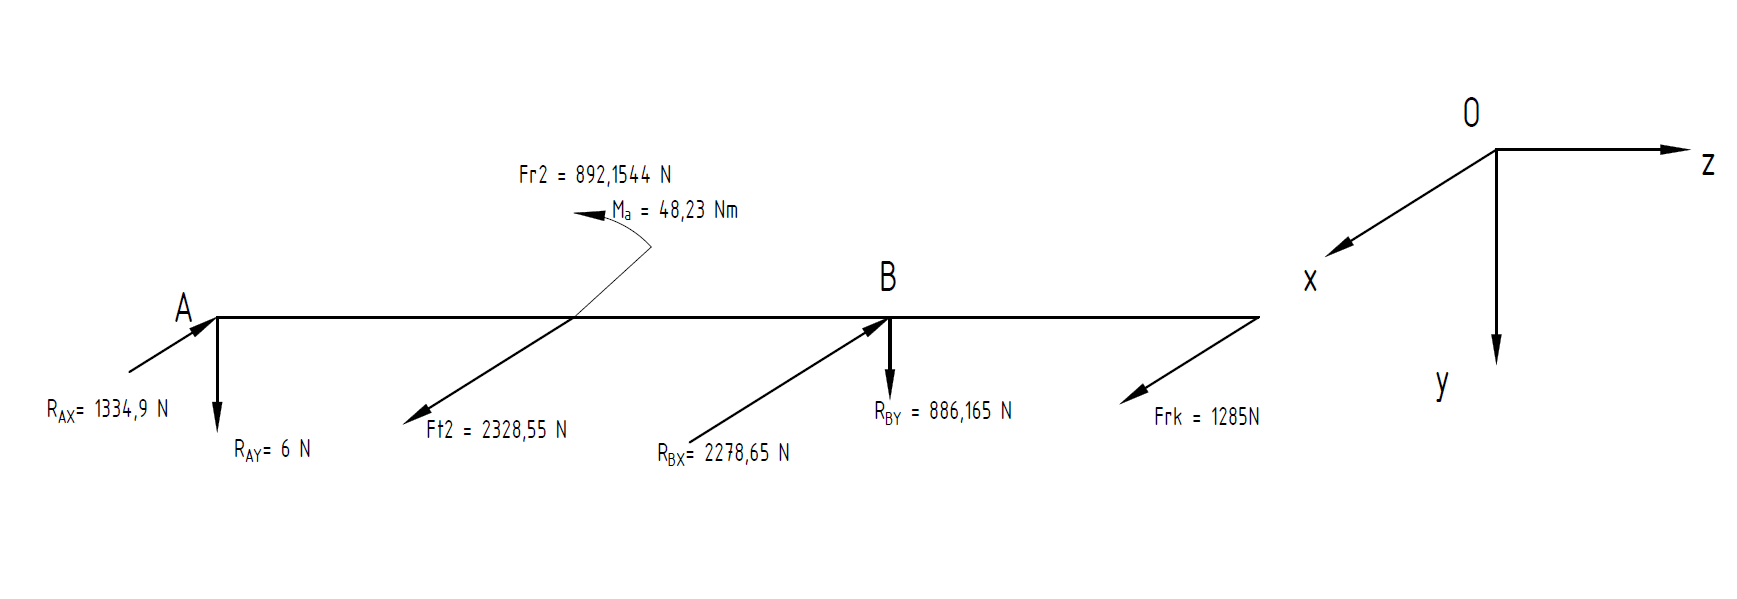
\includegraphics[width=1\textwidth]{pictures/tinholan2.png}
\end{figure}
Xác định phản lực tại các vị trí A và B:
\[
    F_{rA} = \sqrt{R_{AX}^2 + R_{AY}^2} = \sqrt{1334,9^2 + 6^2} = 1334,9N
\]
\[
    F_{rB} = \sqrt{R_{BX}^2 + R_{BY}^2} = \sqrt{2278,65^2 + 886,165^2} = 2444,9N
\]
Tại vị trí B có lực tập trung lớn hơn nên ta chọn ổ lăn theo vị trí B của trục II.
\[
    \frac{F_a}{F_r} = \frac{765,588}{2444,9} = 0,313
\]
Vì $0,3 < \frac{F_a}{F_r} = 0,36 < 0,7$ nên ta chọn loại ổ bi đỡ là ổ bi đỡ chặn 1 dãy. \\
Ta có đường kính trục tại ổ lăn: d = 45mm \\
$\Rightarrow$ Chọn ổ lăn loại ổ bi đỡ chặn, cỡ siêu nhẹ có ký hiệu 46109 với $C = 17300N$ và $C_o = 13700N$.
\begin{figure}[H]
    \centering
    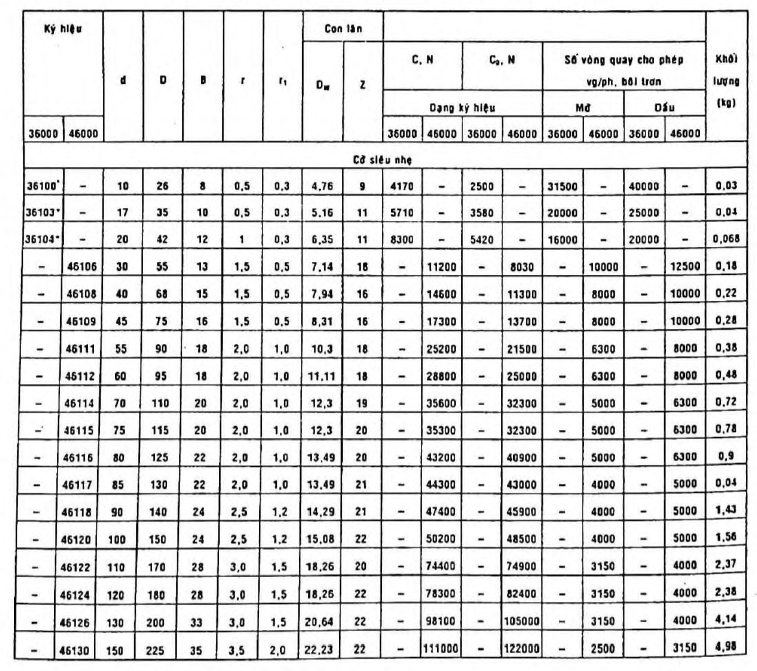
\includegraphics[width=1\textwidth]{pictures/chono2.png}
    \caption{Tiêu chuẩn chọn ổ đỡ chặn cỡ siêu nhẹ}
\end{figure}
\subsection{Tính ổ lăn theo khả năng tải trọng}
\subsubsection*{Chọn các hệ số}
\begin{itemize}
    \item Chọn hệ số $K_\alpha = 1$ do tải trọng tĩnh.
    \item Chọn hệ số $K_t = 1$ do làm việc ở nhiệt độ thường.
    \item Chọn hệ số $V = 1$ do vòng trong quay.\\
    Chọn hệ số X và Y: \\
    $\frac{F_a}{C_o} = \frac{765,588}{13700} = 0,056 \Rightarrow$ chọn e = 0,37.\\
    $\frac{F_a}{VF_r} = \frac{765,588}{1.2444,9} = 0,313 < e = 0,37$ nên chọn X = 1 và Y = 0.
\end{itemize}
\subsubsection*{Thời gian làm việc tính bằng triệu vòng quay}
\[
    L = \frac{60L_hn}{10^6} = \frac{60.6.280.8.2.76,6}{10^6} = 123,54 
\]
\subsubsection*{Tải trọng quy ước tác dụng lên ổ lăn}
\[
    Q = (XVF_r+YF_\alpha)K_\sigma K_\tau = (1.1.3213,53 + 0.765,588).1.1 = 3213,53N
\]
\[
    C_t = Q\sqrt[m]{L} =3213,53\sqrt[3]{123,54} = 3213,53.11,5 = 160005N
\]
Vì $C_t < C = 17300N$ nên việc chọn cỡ siêu nhẹ là hợp lý.
\begin{center}
\begin{tabular}{|c|c|c|c|c|c|c|c|}
    \hline
       \textbf{Ký hiệu} & \textbf{d, mm} & \textbf{D, mm} & \textbf{B, Nm} & \textbf{r, mm} & \textbf{C, N} & \textbf{$C_o$, N} & \textbf{$L_h$, giờ} \\
    \hline
    46109 & 45 & 75 & 16 & 1,5 & 17300 & 13700 & 26880 \\
    \hline
\end{tabular}
\end{center}
\cleardoublepage
    % \section{Chọn dầu bôi trơn cho hộp giảm tốc}
Ta có công thức:
\[
    X_{br} = \frac{10^{-5}H_{HV}\sigma_H^2}{v} = \frac{10^{-5}.260.314,887^2}{1,38} = 186,812
\]
Trong đó: 
\begin{itemize}
    \item $v = 1,38 m/s$
    \item $H_{HV} = 260MPa$
    \item   $\sigma_H = 314,887MPa$
\end{itemize}
Theo đồ thị hình 13.9a/505, ta chọn dầu bôi trơn có $v_{50} = 73 cSt$. Khi đó độ nhớt ở nhiệt độ $40^oC$ là $v_{40} = v_{50}(\frac{40}{50})^3 = 37,376 cSt$.
\begin{figure}[H]
    \centering
    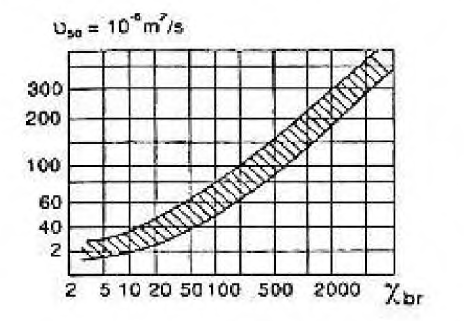
\includegraphics[width=0.4\textwidth]{pictures/nhot1.png}
    \caption{Sự phụ thuộc độ nhớt v theo x của bánh răng}
\end{figure}
Do đó theo bảng 13.1 ta chọn dầu bôi trơn ISO VG 46.
\begin{figure}[H]
    \centering
    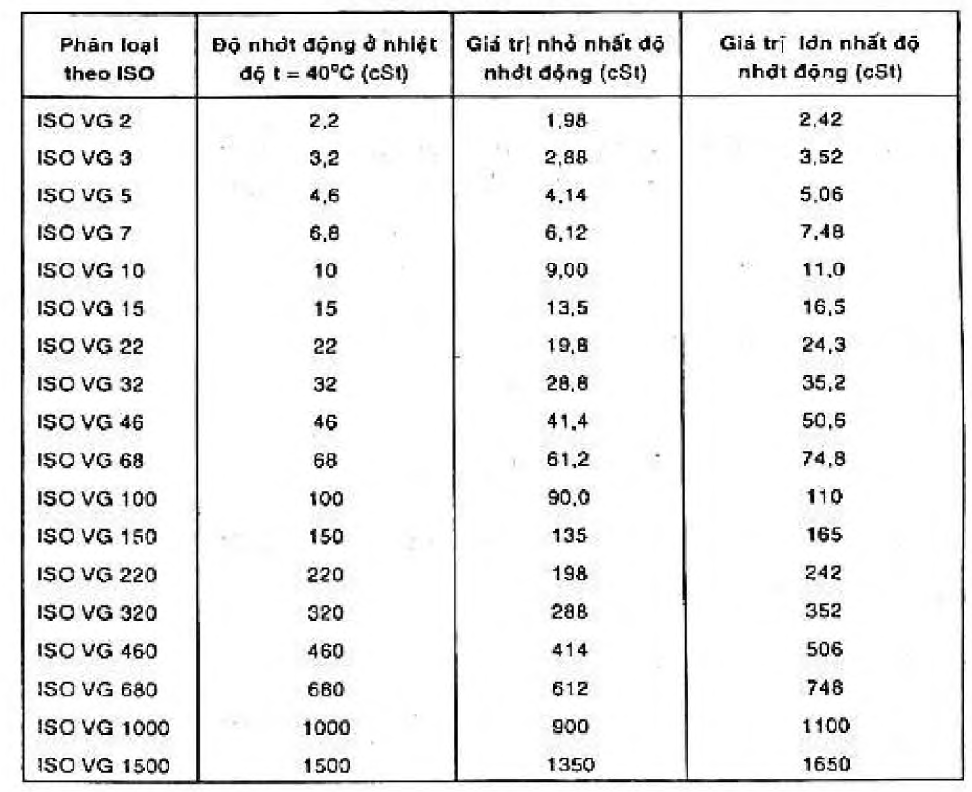
\includegraphics[width=0.5\textwidth]{pictures/nhot2.png}
    \caption{Dầu bôi trơn ISO VG}
\end{figure}
\cleardoublepage
    % \section{Thiết kế nối trục}
Chọn vật liệu chốt - thép C45 với ứng suất uốn cho phép $[\sigma_F] = 70MPa$, ứng suất dập giữa chốt và ống $[\sigma_d] = 3MPa$. \\ 
Sử dụng nối trục đàn hồi theo yêu cầu của bài toán với các thông số như sau:\\
Momen truyền qua nối trục: T = 385,5 Nm \\
Đường kính trục $d_2 = 45mm$\\
\begin{figure}[H]
    \centering
    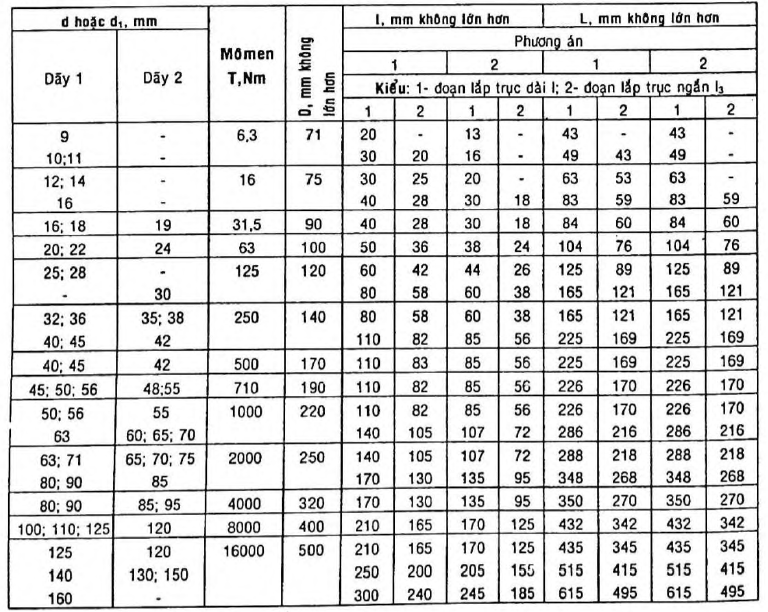
\includegraphics[width=0.8\textwidth]{pictures/noitruc.png}
    \caption{Các kích thước chính chọn nối trục vòng đàn hồi}
\end{figure}
\begin{figure}[H]
    \centering
    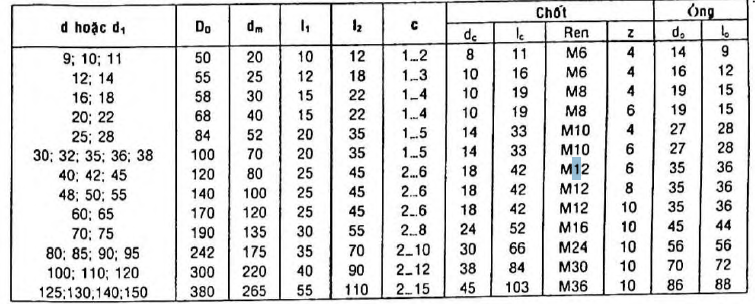
\includegraphics[width=0.8\textwidth]{pictures/noitruc2.png}
    \caption{Các kích thước phụ chọn nối trục vòng đàn hồi}
\end{figure}
Theo phụ lục ta chọn nối trục đàn hồi có: 
\begin{center}
\begin{tabular}{|c|c|c|c|c|c|c|c|c|c|c|c|}
    \hline
    d & $D_0 $  & $d_m$  & $l_1$  & $l_2$  & C  & $d_c$  & $l_c$  & Ren  & z  & $d_0$  & $l_0$ \\
    \hline
    45 & 120 & 80 & 25 & 45 & 3 & 18 & 42 & M12 & 6 & 35 & 36 \\
    \hline
\end{tabular}
\end{center}
Chọn vật liệu chốt thép C45 với ứng suất uốn cho phép, ứng suất trượt giữa chốt 
và ống là $[\sigma_d] =3MPa$ \\
Theo bảng 14.1 chọn chế độ làm việc K = 1,5.
\begin{figure}[H]
    \centering
    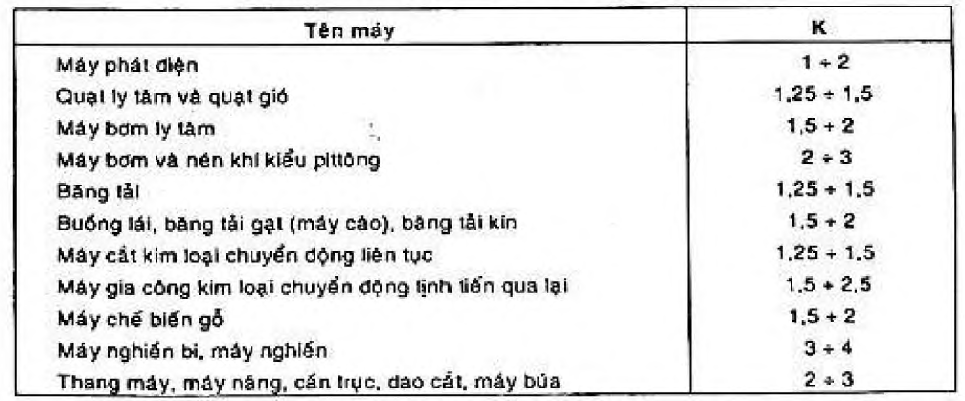
\includegraphics[width=1\textwidth]{pictures/hesolamviec.png}
    \caption{Hệ số làm việc K}
\end{figure}

Kiểm tra độ bền uốn:
\[
    \sigma_F = \frac{32KT.10^3.l_c}{\pi d_c^3.D_0.z} = \frac{32.1,5.385,5.10^3.42}{\pi.18^3.120.6} = 58,9MPa < [\sigma_F] = 70MPa
\]
\hspace*{0,82cm}Kiểm tra độ bền dập:
\[
    \sigma_d = \frac{2KT.10^3}{z.D_0.d_c.l_0}  = \frac{2.1,5.385,5.10^3}{6.120.18.36} = 2,48MPa < [\sigma_d] = 3MPa
\]
$\Rightarrow$ Thỏa mãn điều kiện bền uốn và bền dập.
\cleardoublepage
    \section{Tính bộ phận công tác}
\subsection{Tính bước của trục vít tải}
\begin{itemize}
    \item Ta chọn vật liệu là Inox 304 vì nó có độ bền cao, khả năng chống ăn mòn tốt phù hợp với môi trường làm việc của máy ép bùn.
    \item Ta sử dụng vít tải quay chậm để vận chuyển vật liệu theo phương nằm ngang. 
    \item Khi trục vít quay thì vật liệu được nâng lên và cả khối vật liệu bị nghiêng đi một góc $\varphi $ như hình dưới, tại đó trọng lượng của vật liệu sẽ cân bằng với lực ma sát của vật liệu với thành máy.
\end{itemize}
\begin{figure}[H]
    \centering
    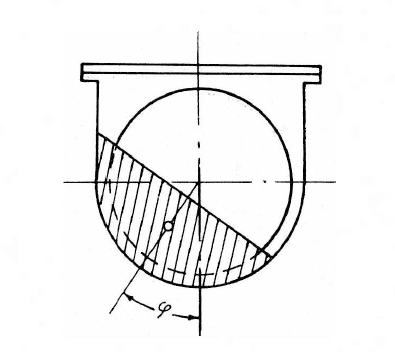
\includegraphics[width=0.5\textwidth]{pictures/vittai1.png}
\end{figure}
% \begin{itemize}
%     \item Chọn góc nghiêng tự nhiên của bùn ở trạng thái tĩnh $\varphi_o = 30^\circ$
%     \item Góc nghiên của khối vật liệu (bùn) $\varphi = 0.7 \varphi_o = 21^\circ$
%     \item Điều kiện để vật liệu trượt được là góc nghiêng của vít tải phải có giá trị nhỏ hơn giá trị giới hạn và giá trị giới hạn của góc nâng của trục vít $\alpha$ được xác định từ quan hệ sau: 
% \end{itemize}
% \[
%     tan(\alpha + \varphi_1) = \frac{sin\varphi}{f_2\cdot cos \varphi + tan\beta}
% \]
% \[
%     tan(\alpha + 30.96) = \frac{\sin21}{0.6\cdot cos21 + tan0}
% \]
% \[
%     \Rightarrow \alpha = 1.65^\circ
% \]
% Trong đó: 
% \begin{itemize}
%     \item $f_1 = 0.6$: hệ số ma sát giữa bùn và cánh vít
%     \item $f_2 = 0.6$: hệ số ma sát giữa bùn và thành máy
%     \item $\varphi_1 = \arctan f_1 = 30.96^\circ$: góc ma sát của vật liệu với cánh vít 
%     \item $\varphi = 21$: góc nghiêng cân bằng của vật liệu (bùn)
%     \item $\beta = 0$: góc nghiêng của vít tải so với mặt phẳng ngang
% \end{itemize}
% Khi đó góc nâng thực tế của trục vít lấy bằng:
% \[
%     \alpha_t = 0.8\alpha = 0.8 \cdot 1.65 = 1.32^\circ
% \]
% \[
%     S=\pi\cdot D\cdot tan\alpha_t = \pi \cdot 0.225 \cdot tan1.32 = 0.01629 (m) = 16.29 (mm)
% \]
\begin{itemize}
    \item Bước của trục vít (hay khoảng cách giữa các cánh vít) đối với vật liệu dạng bột hoặc hạt nhỏ được xác định là:
    \[
        S = (0.7 \div 1)D = 0.8 \cdot 225 = 180 (mm) 
    \]
\end{itemize}
\subsection{Diện tích tiết diện ngang do vật liệu chiếm trong thành máy}
\[
    F = \frac{\pi\cdot D^2}{4}\mu \cdot K = \frac{\pi\cdot 0.225^2}{4}\cdot 0.35\cdot 1 = 0.0139 (m^2)
\]
Trong đó: 
\begin{itemize}
    \item D = 225 mm, là đường kính của vít tải
    \item $\mu$ là hệ số chứa vật liệu trong thành máy. Với vật liệu dạng bột ta chọn $\mu = 0.35$
    \item K là hệ số chỉ sự giảm tiết diện do góc nghiêng đặt vít tải. Với góc nghiêng bằng $0^{\circ}$ ta chọn $K = 1$
\end{itemize}
\subsection{Vận tốc chuyển vật liệu dọc theo trục vít}
\[
    v = \frac{S\cdot n_{ct}}{60} = \frac{0.18\cdot 118.85}{60} = 0.356 (m/s)
\]
Trong đó: 
\begin{itemize}
    \item $S = 180 mm$: bước của vít tải
    \item $n_{ct} = 118.85$ vòng/phút: số vòng quay của trục vít tải
\end{itemize}
\subsection{Xác định năng xuất máy}
\[
    Q = 3600F\cdot v\cdot \rho = 3600\cdot 0.0139\cdot 0.356\cdot 1000 = 17814.24 (kg/h)
\]
Trong đó:
\begin{itemize}
    \item $F = 13916.27 mm^2$: diện tích ngang do vật liệu chiếm trong thành máy
    \item $v = 0.356$ m/s: vận tốc chuyển vật liệu dọc theo trục vít
    \item $\rho = 1000$ kg/m$^3$: khối lượng riêng của bùn
\end{itemize}


\end{document}